
% this file is called up by thesis.tex
% content in this file will be fed into the main document
% ----------------------- paths to graphics ------------------------

% change according to folder and file names
\ifpdf
    \graphicspath{{8/figures/PNG/}{8/figures/PDF/}{8/figures/}}
\else
    \graphicspath{{8/figures/EPS/}{8/figures/}}
\fi


\chapter{Regulated Hydraulic Turbines}

In order to increase the operational range of a hydraulic turbine in terms of allowed flowrates Q and hydraulic heads H, the concept of regulation is frequently used. A regulated hydraulic turbine is a turbine in which the stator or rotor or both have adjustable blades. An adjustable blade can rotate around a predefined axis by means of an appropriate mechanism. 


\section{Single-Regulated Turbines}
\label{single.regulated}

Hydraulic turbines that have a single row of adjustable blades (usually the stator blades) are called single-regulated turbines (fig.\ \ref{signle}). Typical examples of single-regulated turbines are Francis turbines, axial fixed-blade propeller turbines with adjustable stator blades and the so-called semi-Kaplan concept with fixed stator and adjustable rotor blades, \cite{papanto,drtina1999hydraulic}.  
Though the rotation angle $\alpha^j$ of the adjustable blades might be handled as one additional design variable per operating point $j$, a different approach is proposed in this thesis. 
                 

Regarding its application to single-regulated turbines, the proposed method has the advantage of: (a) removing the burden of computing the appropriate $\alpha^j$ angles by the EA and (b) eliminating the need to impose additional constraints to ensure operation at the desirable operating points. Instead, it is sufficient to ensure, through an iterative procedure,  that each candidate solution computes the appropriate $\alpha^j$ angles for operating at the desirable points. Quality metrics are then computed and the evolution continues as presented in Chapter 5.  To do so, evaluation procedure is modified by including the computation of the right $\alpha^j$ value for each operating point $j$. In specific, for each candidate solution and for each operating point: 

\begin{itemize}
\item[]{\bf Step 1:}  (Initialization) 
\begin{itemize}
	\item[]{\bf Step 1a:} (Initialize $\alpha$) Sets the iteration counter to $i=0$ and $\alpha_i=\alpha _0$, where $\alpha _0$ a user-defined value.
	\item[]{\bf Step 1b:} (First Step) Sets $i \! = \! 1$ and $\Delta \alpha \! = \! \Delta \alpha_0$, where $\Delta \alpha_0$ the user-defined increment and defines 
\begin{eqnarray}
	\alpha_1={\left\{ 
	\begin{array}{ll}
    \alpha_0 - \Delta \alpha_0 ~~,\mbox{if $(Q < Q_{required})$ or ($H > H_{required})$}\\
	\alpha_0 + \Delta \alpha_0 ~~,\mbox{if $(Q > Q_{required})$ or $(H < H_{required})$}\\
    \end{array} \right. }
    \label{step0}
\end{eqnarray}  
By definition, $\alpha=0^o$ corresponds to the fully open stator position.
\end{itemize}

\item[]{\bf Step 2:}  (Gradient Computation) Sets $i=i+1$. Computes derivatives $\frac{\partial(Q-Q{required})}{\partial \alpha}$ or $\frac{\partial(H-H{required})}{\partial \alpha}$, depending on the boundary conditions employed  in the flow solver. Finite-difference quotients such as the following ones 
\begin{eqnarray}
	\frac{\partial(Q-Q_{required})}{\partial \alpha}=\frac{(Q_{i-1}-Q_{required})-(Q_{i-2}-Q_{required})}{\alpha_{i-1}- \alpha_{i-2}}
\end{eqnarray}  
are used. 

\item[]{\bf Step 3:}  (Update $\alpha$) Based on the Newton-Raphson method, updates $\alpha$ as follows
\begin{eqnarray}
	\alpha_{i}=\alpha_{i-1} - \eta \frac{Q_{i-1}-Q_{required}} {\frac{\partial(Q-Q_{required})}{\partial \alpha}}  
\end{eqnarray}  
where $\eta$ is a user-defined relaxation factor. 

\item[]{\bf Step 3:} (Convergence Check) Stops if $|Q_{i}-Q_{required}|<\Delta Q^*$, where $\Delta Q^*$ a user-defined threshold value; otherwise, continues from step 2. 
\end{itemize}  

This algorithm can be scaled to any number of operating points, in case of multi-operating point design problems.     


\begin{figure}[h!]
\centering
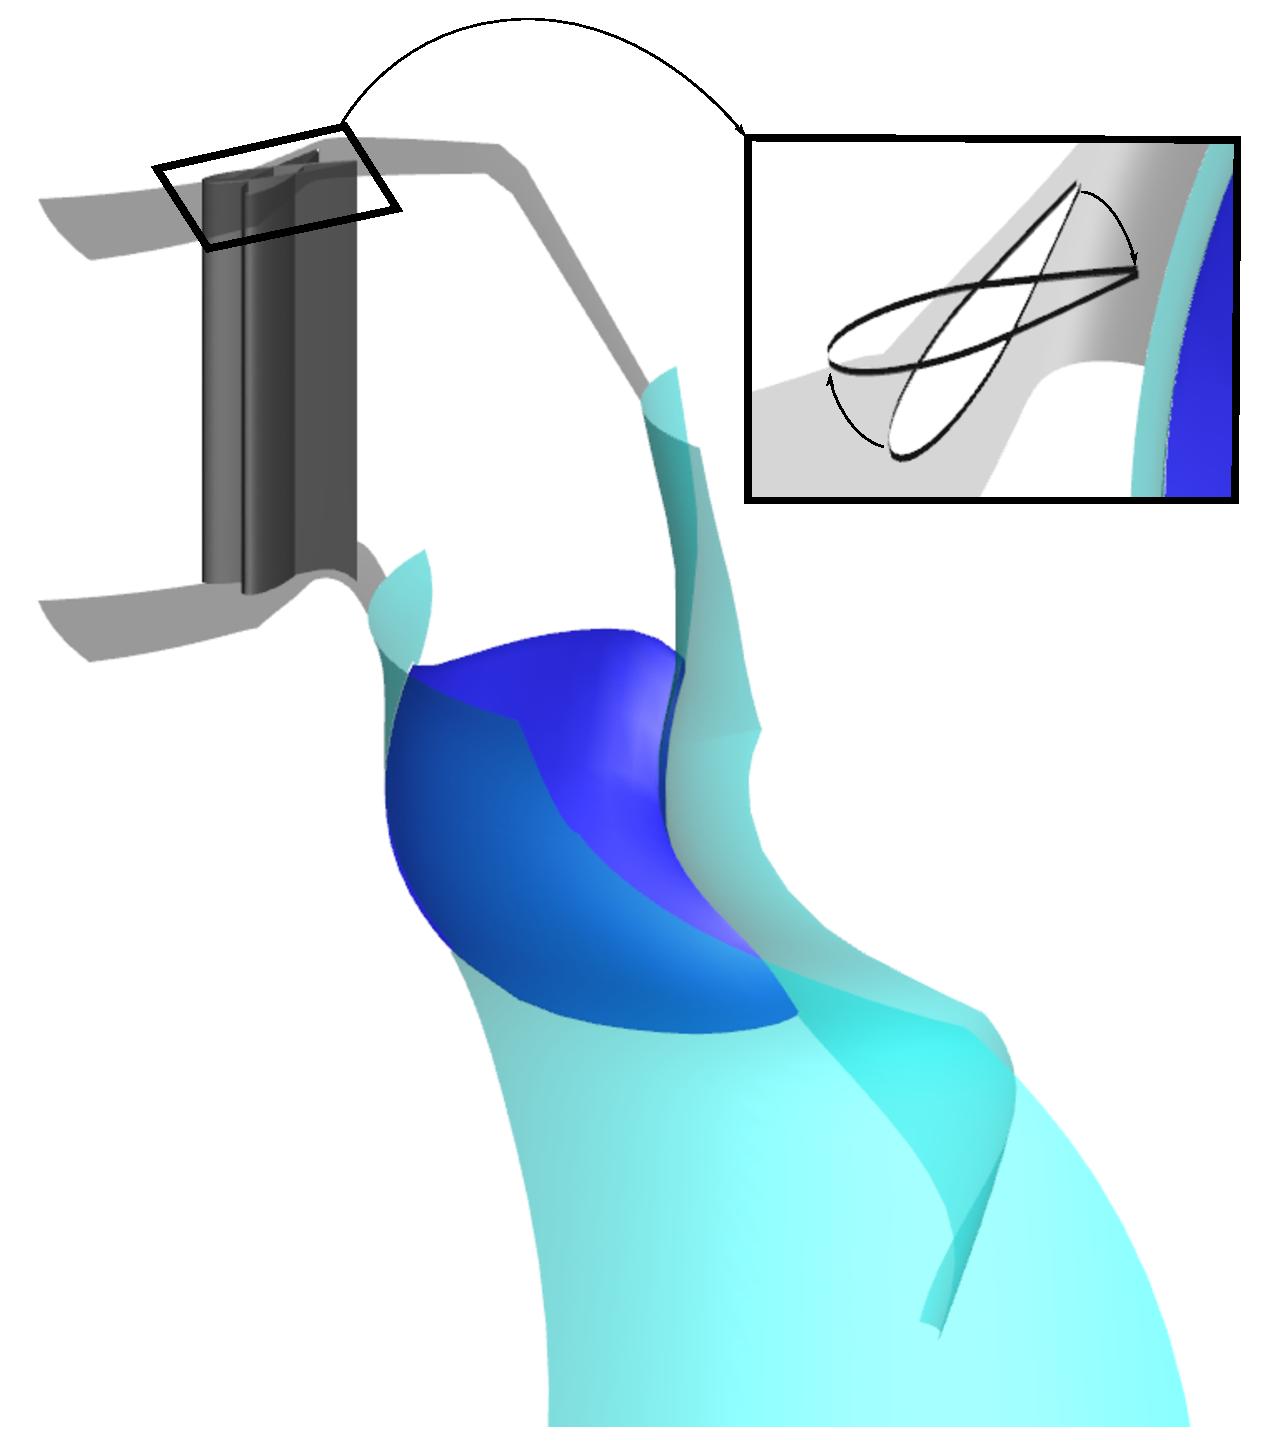
\includegraphics[width=.8\textwidth]{SINGLE.eps}
\caption{Single-regulated (axial) turbine.  The adjustable stator blades are shown in grey whereas the non-adjustable rotor blades in blue.}
\label{signle}
\end{figure}



\FloatBarrier  
\section{Double-Regulated Turbines}

Hydraulic turbines that have two rows of adjustable blades (rotor and stator, fig.\ \ref{double}) are called double-regulated turbines,  \cite{papanto,drtina1999hydraulic}. A typical example is the Kaplan turbine.  
In double-regulated turbines, the stator rotation angle is denoted by $\alpha$ (in accordance with what was used before) and  the rotor rotation angle by $\beta$. 

\begin{figure}[h!]
\centering
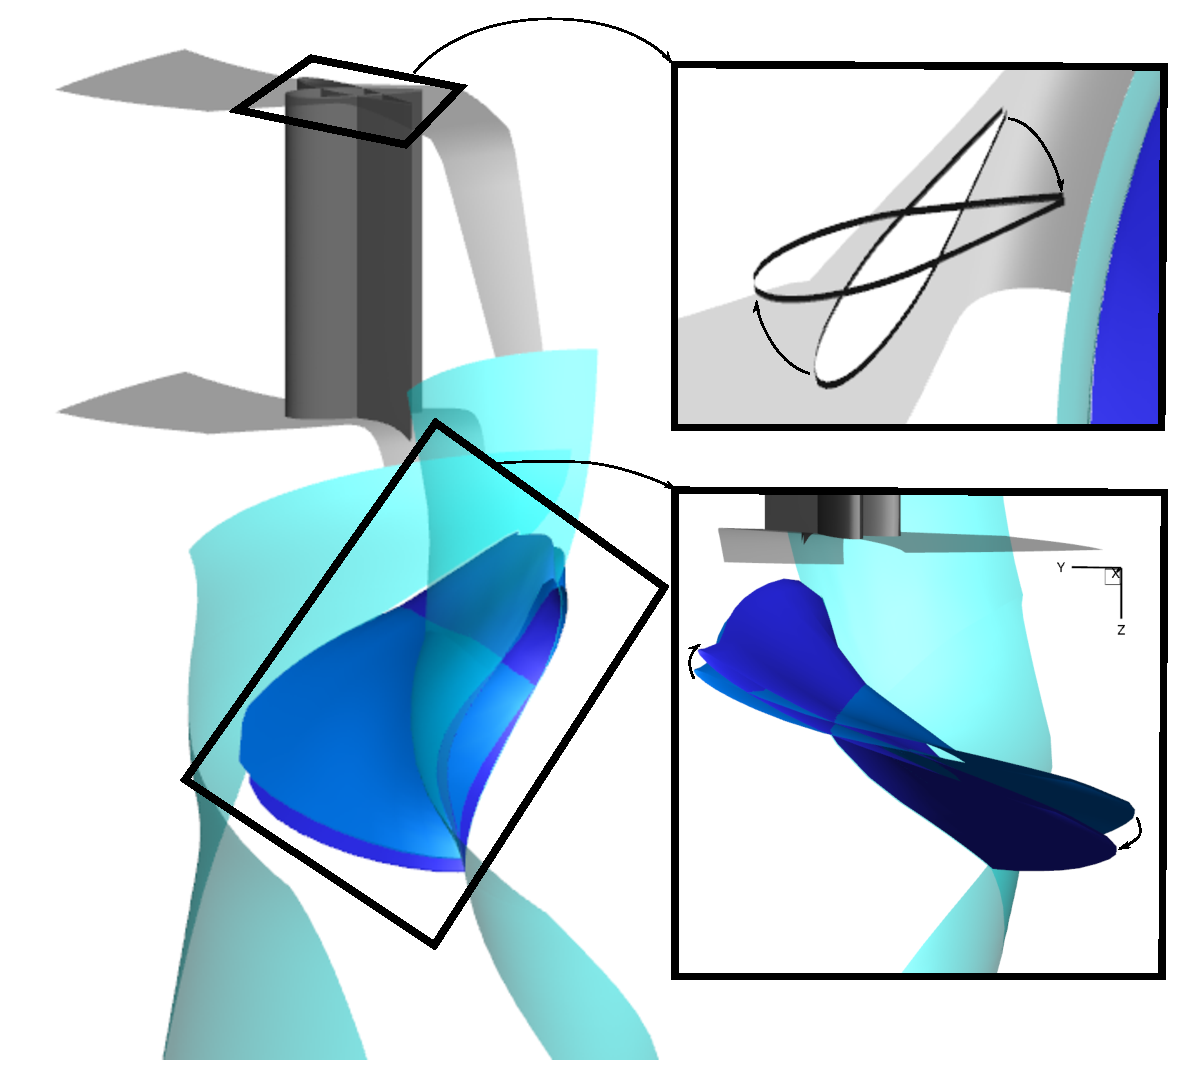
\includegraphics[width=.8\textwidth]{DOUBLE.eps}
\caption{Double-regulated (Kaplan) turbine. In contrast to fig.\ \ref{signle}, the rotor blades (in blue) are also adjustable.}
\label{double}
\end{figure}

To handle the design of double-regulated turbines, the algorithm proposed for the single-regulated ones to compute the $\alpha^j$ angles is used. Over and above, the introduction of $\beta^j$, where $j$ is the operating point counter, as additional design variables takes place. Doing so, the EA overcomes the computation of the $\alpha^j$ angles (as for single-regulated turbines) and undertakes only the search for the optimal $\beta^j$ angles so as to achieve best performance for each operating point. %This can be seen as using $\alpha$ to set the operating point and $\beta$ to ensure operation at the on-cam position.    

% ---------------------------------------------------------------------------
%: ----------------------- end of thesis sub-document ------------------------
% ---------------------------------------------------------------------------



 






